\documentclass[10pt,conference,english,twocolumn]{IEEEtran}
\usepackage[svgnames]{xcolor}
\usepackage{amsmath}
\usepackage{amssymb}
\usepackage{tikz}
\usepackage{pgfplots}
\pgfplotsset{compat=newest}
\usetikzlibrary{positioning}
\usetikzlibrary{shapes.geometric, arrows, decorations.pathreplacing}
\usetikzlibrary{shapes.arrows}
\usetikzlibrary{3d}

\begin{document}

    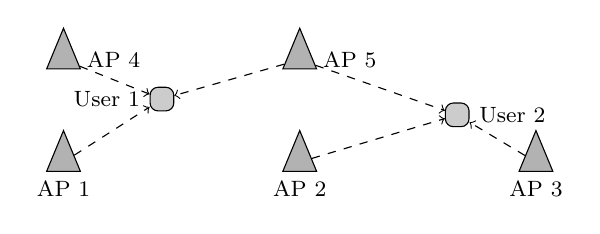
\begin{tikzpicture}
    \tikzstyle{every node}=[font=\footnotesize]
    \tikzstyle{ap}=[isosceles triangle, draw, rotate=90, fill=gray!60, minimum size =.25cm]
    \tikzstyle{user}=[rectangle, draw, fill=gray!40, minimum size =.3cm, rounded corners=0.1cm]

    \node[ap,label={left:AP 1}] (ap1) at (0,0){};
    \node[ap,label={left:AP 2}] (ap2) at (3,0){};
    \node[ap,label={left:AP 3}] (ap3) at (6,0){};
    \node[ap,label={below:AP 4}] (ap4) at (0,1.3){};
    \node[ap,label={below:AP 5}] (ap5) at (3,1.3){};

    \node[user,label={left:User 1}] (u1) at (1.25,0.8){};
    \node[user,label={right:User 2}] (u2) at (5, 0.6){};

    \draw[dashed, ->] (ap1) -- (u1);
    \draw[dashed, ->] (ap4) -- (u1);
    \draw[dashed, ->] (ap5) -- (u1);
    \draw[dashed, ->] (ap2) -- (u2);
    \draw[dashed, ->] (ap5) -- (u2);
    \draw[dashed, ->] (ap3) -- (u2);
\end{tikzpicture}

\end{document}